\documentclass{../../../oss-apphys-exam}
\newcounter{lastmc}

\begin{document}

\gentitle{3}{DYNAMICS, WORK \& ENERGY}

\raggedcolumns

\runningheader{
  \fontfamily{phv}\small
  \textcolor{gray}{AP PHYSICS C: MECHANICS $\blacksquare$}
  \textbf{MULTIPLE-CHOICE QUESTIONS}}{}{}

\begin{multicols*}{2}
  \textbf{Questions \ref{q:2blocks1}--\ref{q:2blocks2}}: Two blocks,
  \SI4{\kilo\gram} and \SI2{\kilo\gram}, are connected by a string. An applied
  force $F$ of magnitude \SI{18}{\newton} pulls the blocks to the left.
  \begin{center}
    \begin{tikzpicture}[scale=.95,thick]
      \fill[pattern=north east lines] (2.5,0) rectangle(9,-.3);
      \draw (2.5,0)--(9,0);
      \draw (7,0) rectangle(8,1) node[midway]{2 kg};
      \draw (4,0) rectangle(6,1) node[midway]{4 kg};
      \draw (6,.5)--(7,.5);
      \draw[->] (4,.5)--(3,.5) node[left]{\SI{18}\newton};
    \end{tikzpicture}
  \end{center}

  \begin{questions}
    \question The acceleration of the \SI4{\kilo\gram} block is
    \begin{choices}
      \choice\SI2{\metre\per\second\squared}
      \choice\SI3{\metre\per\second\squared}
      \choice\SI4{\metre\per\second\squared}
      \choice\SI{4.5}{\metre\per\second\squared}
      \choice\SI6{\metre\per\second\squared}
    \end{choices}
    \label{q:2blocks1}
    
    \question The tension in the string between the blocks is
    \begin{choices}
      \choice 4 N
      \choice 6 N
      \choice 12 N
      \choice 16 N
      \choice 18 N
    \end{choices}
    \label{q:2blocks2}

        \uplevel{
      \textbf{Questions \ref{3blks1}--\ref{3blks2}}
      
      Three blocks of mass \SI3{\kilo\gram}, \SI2{\kilo\gram}, and
      \SI1{\kilo\gram} are pushed along a horizontal frictionless plane by a
      force of \SI{24}{\newton} to the right, as shown.
      \begin{center}
        \begin{tikzpicture}[scale=.9]
          \fill[pattern=north east lines] rectangle(8,-.3);
          \begin{scope}[thick]
            \draw (0,0)--(8,0);
            \draw (2,0) rectangle(4,1.5) node[midway]{3 kg};
            \draw (4,0) rectangle(5.5,1.3) node[midway]{2 kg};
            \draw (5.5,0) rectangle(6.5,1.1) node[midway]{1 kg};
            \draw[->](0,.75)--(2,.75) node[midway,above]{24 N};
          \end{scope}
        \end{tikzpicture}
      \end{center}
    }

    \question The acceleration of the \SI{2}{\kilo\gram} block is
    \begin{choices}
      \choice\SI{144}{\metre\per\second\squared}
      \choice\SI{72}{\metre\per\second\squared}
      \choice\SI{12}{\metre\per\second\squared}
      \choice\SI6{\metre\per\second\squared}
      \choice\SI4{\metre\per\second\squared}
    \end{choices}
    \label{3blks1}
    
    \question The force that the \SI2{\kilo\gram} block exerts on the
    \SI1{\kilo\gram} block is
    \begin{choices}
      \choice\SI2\newton
      \choice\SI4\newton
      \choice\SI6\newton
      \choice\SI{24}\newton
      \choice\SI{144}\newton
    \end{choices}
    \label{3blks2}
    \columnbreak
    
    \uplevel{
      \textbf{Questions \ref{q:pulley1}--\ref{q:pulley2}}: A system consists of
      two blocks having masses of \SI2{\kilo\gram} and \SI1{\kilo\gram}. The
      blocks are connected by a string of negligible mass and hung over a light
      pulley, and then released from rest.
      \begin{center}
        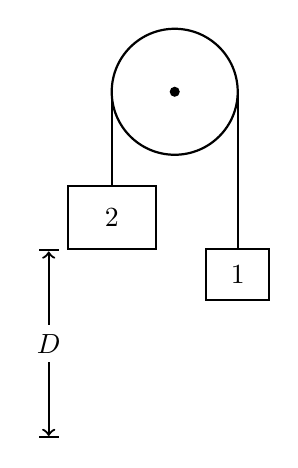
\begin{tikzpicture}[scale=.8]
          \begin{scope}[thick]
            \draw circle (1);
            \fill circle (.08);
            \draw (1,0)--(1,-2.5);
            \draw (.5,-2.5) rectangle (1.5,-3.3)
            node[midway]{\SI1{\kilo\gram}};
            \draw (-1,0)--(-1,-1.5);
            \draw (-1.7,-1.5) rectangle (-.3,-2.5)
            node[midway]{\SI2{\kilo\gram}};
            \draw[|<->|] (-2,-2.5)--(-2,-5.5) node[midway,fill=white]{$D$};
          \end{scope}
        \end{tikzpicture}
      \end{center}
    }

  \question The acceleration of the \SI2{\kilo\gram} block is most nearly
    \begin{choices}
      \choice $\dfrac29g$
      \choice $\dfrac13g$
      \choice $\dfrac12g$
      \choice $\dfrac23g$
      \choice $g$
    \end{choices}
    \label{q:pulley1}
    
    \question The speed of the \SI2{\kilo\gram} block after it has descended a
    distance $D$ is most nearly
    \begin{choices}
      \choice $\sqrt{\dfrac{4gD}3}$
      \choice $\sqrt{\dfrac{2gD}3}$
      \choice $\sqrt{\dfrac{gD}3}$
      \choice $\sqrt{\dfrac{gD}2}$
      \choice $\sqrt{\dfrac{4gD}6}$
    \end{choices}
    \label{q:pulley2}
    \columnbreak
    
    \uplevel{
      \textbf{Questions \ref{plane1}--\ref{plane2}}: A \SI{10}{\newton} block
      sits atop an inclined plane in the shape of a right triangle of sides
      \SI3\metre, \SI4\metre, and \SI5\metre, as shown. The block is allowed to
      slide down the plane without friction.
      \begin{center}
        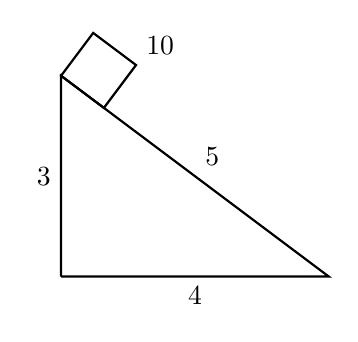
\begin{tikzpicture}[scale=.85]
          \begin{scope}[thick]
            \draw(0,0)--(4,0) node[midway,below]{\SI4\metre}
            --(0,3) node[midway,above right]{\SI5\metre}
            --(0,0) node[midway,left]{\SI3\metre};
            \draw[rotate around={-atan(3/4):(0,3)}](0,3) rectangle(.8,3.8)
            node[above right]{\SI{10}\newton};
          \end{scope}
        \end{tikzpicture}
      \end{center}
    }
    
    \question The acceleration of the block is most nearly
    \begin{choices}
      \choice\SI2{\metre\per\second\squared}
      \choice\SI4{\metre\per\second\squared}
      \choice\SI6{\metre\per\second\squared}
      \choice\SI{10}{\metre\per\second\squared}
      \choice\SI{12}{\metre\per\second\squared}
    \end{choices}
    \label{plane1}
    
    \question The normal force exerted on the block by the plane is most nearly
    \begin{choices}
      \choice\SI2\newton
      \choice\SI4\newton
      \choice\SI6\newton
      \choice\SI{8}\newton
      \choice\SI{10}\newton
    \end{choices}
    \label{plane2}
    \columnbreak
    
    \uplevel{
      \textbf{Questions \ref{stacked1}--\ref{stacked2}}: A block of mass
      \SI2{\kilo\gram} rests on top of a larger block of mass \SI4{\kilo\gram}.
      The larger block slides without friction on a table, but the surface
      between the two blocks is not frictionless. The coefficient of friction
      between the two blocks is $0.2$. A horizontal force $\vec F$ is applied
      to the \SI4{\kilo\gram} mass.
      \begin{center}
        \begin{tikzpicture}[scale=.95]
          \fill[pattern=north east lines] (3,0) rectangle(9,-.3);
          \draw[thick] (3,0)--(9,0);
          \draw[thick] (5,1) rectangle(6,2) node[midway]{\SI2{\kilo\gram}};
          \draw[thick] (4,0) rectangle(7,1) node[midway]{\SI4{\kilo\gram}};
          \draw[thick,->] (7,.5)--(8,.5) node[right]{$\vec F$};
        \end{tikzpicture}
      \end{center}
    }

    \question What is the maximum force that can be applied such that there is
    no relative motion between the two blocks?
    \begin{choices}
      \choice zero
      \choice \SI1\newton
      \choice \SI2\newton
      \choice \SI4\newton
      \choice \SI{12}\newton
    \end{choices}
    \label{stacked1}
    
    \question What is the acceleration of the \SI2{\kilo\gram} block relative
    to the \SI4{\kilo\gram} block if a force is applied to the 4-kg block that
    causes the \SI4{\kilo\gram} block to accelerate at
    \SI3{\metre\per\second\squared} to the right?
    \begin{choices}
      \choice\SI1{\metre\per\second\squared} to the right
      \choice\SI1{\metre\per\second\squared} to the left
      \choice\SI2{\metre\per\second\squared} to the right
      \choice\SI2{\metre\per\second\squared} to the left
      \choice zero
    \end{choices}
    \label{stacked2}
    \setcounter{lastmc}{\value{question}}
  \end{questions}
\end{multicols*}
\newpage


\runningheader{
  \fontfamily{phv}\small
  \textcolor{gray}{AP PHYSICS C: MECHANICS $\blacksquare$}
  \textbf{FREE-RESPONSE QUESTIONS}}{}{}


\begin{center}
  \cpic{.5}{amusement}
\end{center}
  
% THIS IS TAKEN FROM THE 2011 AP PHYSICS C FREE-RESPONSE QUESTION MECH 2
\begin{questions}
  \setcounter{question}{\value{lastmc}}
  \question An amusement park ride features a passenger compartment of mass $M$
  that is released from rest at point $A$, as shown in the figure above, and
  moves along a track to point $E$. The compartment is in free fall between
  points $A$ and $B$, which are a distance of $3R/4$ apart, then moves along
  the circular arc of radius $R$ between points $B$ and $D$. Assume the track is
  frictionless from point $A$ to point $D$ and the dimensions of the passenger
  compartment are negligible compared to $R$.
  \begin{parts}
    \part On the dot below that represents the passenger compartment,
    \textbf{draw} and \textbf{label} the forces (not components) that act on
    the passenger compartment  when it is at point $C$, which is at an angle
    $\theta$ from point $B$.
    \label{diagram-a}
    \begin{center}
      \vspace{.1in}
      \begin{tikzpicture}
        \fill circle (.15);
        \draw[rotate=35,dashed,thick] (0,2)--(0,-2);
      \end{tikzpicture}
    \end{center}
    
    \part In terms of $\theta$ and the magnitudes of the forces drawn in part
    (\ref{diagram-a}), \textbf{derive} an expression for the magnitude of the
    centripetal force acting on the compartment at point $C$. If you need to
    draw anything besides what you have shown in part (\ref{diagram-a}) to
    assist in your solution, use the space below. Do NOT add anything to the
    figure in part (\ref{diagram-a}).
    \vspace{\stretch1}
    
    \part\textbf{Derive} an expression for the speed $v_D$ of the passenger
    compartment as it reaches point $D$ in terms of $M$, $R$, and fundamental
    constants, as appropriate.
    \vspace{\stretch1}
    \newpage
    
    \uplevel{
      A force acts on the compartment between points $D$ and $E$ and brings it
      to rest at point $E$.
    }
    
    \part If the compartment is brought to rest by friction, \textbf{calculate}
    the numerical value of the coefficient of friction $\mu$ between the
    compartment and the track.
    \vspace{\stretch1}
    
    \uplevel{
      Now consider the case in which there is no friction between the
      compartment and the track, but instead the compartment is brought to rest
      by a braking force $-kv$, where $k$ is a constant and $v$ is the
      velocity of the compartment. Express all algebraic answers to the
      following in terms of $M$, $R$, $k$, $v_D$, and fundamental constants, as
      appropriate.
    }

    \part\textbf{Write}, but do NOT solve, the differential equation for $v(t)$.
    \vspace{\stretch1}
    \label{diffeq}
    
    \part\textbf{Solve} the differential equation you wrote in part
    (\ref{diffeq}).
    \vspace{\stretch1}
    
    \part On the axes below, \textbf{sketch} a graph of the magnitude of the
    acceleration of the compartment as a function of time. On the axes,
    explicitly \textbf{label} any intercepts, asymptotes, maxima, or minima with
    numerical values or algebraic expressions, as appropriate.
    \begin{center}
      \vspace{.2in}
      \begin{tikzpicture}[scale=1.5,very thick,->]
        \draw (0,0)--(7,0) node[right]{$t$};
        \draw (0,0)--(0,3) node[above]{$a$};
      \end{tikzpicture}
    \end{center}
  \end{parts}
  \newpage

  % TAKEN FROM THE 2009 AP PHYSICS C MECH EXAM FREE-RESPONSE QUESTION MECH 3
  \uplevel{
    \cpic{.62}{pulley1}
  }
  \question A block of mass $M/2$ rests on a frictionless horizontal table, as
  shown above. It is connected to one end of a string that passes over a
  massless pulley and has another block of mass $M/2$ hanging from its other
  end. The apparatus is released from rest.
  \begin{parts}
    \part\textbf{Derive} an expression for the speed $v_h$ of the hanging block
    as a function of the distance $d$ it descends.
    \label{vh}
    \vspace{\stretch1}
    
    \uplevel{
      Now the block and pulley system is replaced by a uniform rope of length
      $L$ and mass $M$, with one end of the rope hanging slightly over the edge
      of the frictionless table. The rope is released from rest, and at some
      time later there is a length $y$ of rope hanging over the edge, as shown
      below. Express your answers to parts (b), (c), and (d) in terms of
      $y$, $L$, $M$, and fundamental constants.
      \cpic{.45}{rope1}
    }
    
    \part\textbf{Derive} an expression for the force of gravity on the hanging
    part of the rope as a function of $y$.
    \vspace{\stretch1}
    \newpage
    
    \part\textbf{Derive} an expression for the work done by gravity on the rope
    as a function of $y$, assuming $y$ is initially zero.
    \vspace{\stretch1}
    
    \part\textbf{Derive} an expression for the speed $v_r$ of the rope as a
    function of $y$.
    \label{vr}
    \vspace{\stretch1}
    
    \part The hanging block and the right end of the rope are each allowed to
    fall a distance $L$ (the length of the rope). The string is long enough
    that the sliding block does not hit the pulley. \textbf{Indicate} whether
    $v_h$ from part (\ref{vh}) or $v_r$ from part (\ref{vr}) is greater after
    the block and the end of the rope have traveled this distance.

    \vspace{.2in}
    \underline{\hspace{.5in}} $v_h$ is greater.\hspace{.5in}
    \underline{\hspace{.5in}} $v_r$ is greater.\hspace{.5in}
    \underline{\hspace{.5in}} The speeds are equal.

    \vspace{.2in}\textbf{Justify} your answer.
    \vspace{\stretch2}
  \end{parts}
  \newpage

  \uplevel{
    \cpic{.6}{detectors}
  }
  % TAKEN FROM THE 2021 AP PHYSICS C MECH EXAM SET 2 FREE-RESPONSE QUESTION 1
  \question Students design an experiment using blocks of adjustable mass to
  investigate friction using the setup shown. Block 1 of initial mass
  \SI{.44}{\kilo\gram} is placed on a rough horizontal surface and connected by
  a string to block 2 of initial mass \SI{.20}{\kilo\gram}. The string extends
  over a pulley that has negligible mass and friction, as shown in the figure.
  \begin{parts}
    \part\textbf{Calculate} the minimum value of the coefficient of static
    friction $\mu_s$ that would keep the two-block system at rest.
    \newpage

    \uplevel{
      The coefficient of friction is such that when block 2 is released from
      rest, block 1 travels across the surface. The acceleration of each block
      is recorded with motion detectors 1 and 2, as shown in the figure. The
      data for the motion detectors as functions of time are shown on the
      graphs. For each motion detector, the positive direction is away from the
      detector.
      \begin{center}
        \begin{tikzpicture}[scale=2]
          \node[above] at (.75,2){Motion Detector 1};
          \draw[axes] (0,0)--(1.7,0) node[right]{$t$ [s]};
          \draw[axes] (0,-1.3)--(0,1.5)
          node[above]{$a$ [\si{\metre\per\second\squared}]};
          \draw[step=.125,thin,gray,dotted] (0,-1.3) grid (1.6,1.3);
          \draw[step=.5] (0,-1.3) grid (1.6,1.3);
          \foreach \x in {0.0,0.5,1.0,1.5}
          \node[below] at (\x,-1.3){\small$\x$};

          \foreach \y in {2,1,0,-1,-2} \node[left] at (0,\y/2){\small$\y$};
          \draw[very thick] (0,1.17)--+(1.6,0);
        \end{tikzpicture}
        \hspace{.3in}
        \begin{tikzpicture}[scale=2]
          \node[above] at (.75,2){Motion Detector 2};
          \draw[axes] (0,0)--(1.7,0) node[right]{$t$ [s]};
          \draw[axes] (0,-1.3)--(0,1.5)
          node[above]{$a$ [\si{\metre\per\second\squared}]};
          \draw[step=.125,thin,gray,dotted] (0,-1.3) grid (1.6,1.3);
          \draw[step=.5] (0,-1.3) grid (1.6,1.3);
          \foreach \x in {0.0,0.5,1.0,1.5}
          \node[below] at (\x,-1.3){\small$\x$};

          \foreach \y in {2,1,0,-1,-2} \node[left] at (0,\y/2){\small$\y$};
          \draw[very thick] (0,-1.17)--+(1.6,0);
        \end{tikzpicture}
      \end{center}
    }

    \part On the dots below, which represent the blocks, \textbf{draw} and
    \textbf{label} the forces (not components) that act on each block. Each
    force must be represented by a distinct arrow starting on, and pointing
    away from, the dot.
    \begin{center}
      \begin{tikzpicture}
        \node at (0,1.8){Block 1};
        \node at (7,1.8){Block 2};
        \fill circle (.15);
        \fill (7,0) circle (.15);
      \end{tikzpicture}
    \end{center}
    \vspace{.65in}
    
    \part\textbf{Calculate} the coefficient of kinetic friction $\mu_k$ between
    block 1  and the table.
    \label{mu_k}
    \vspace{\stretch1}
    
    \part Careful measurements determine that the coefficient of kinetic
    friction is larger than the value calculated in part (\ref{mu_k}).
    \textbf{Indicate} whether the following explanation sufficiently account
    for the observed discrepancy
    
    \vspace{.2in}``The horizontal table was not perfectly level before the
    experiment was conducted. The observed difference in the angle accounts for
    the difference in the expected and calculated values of $\mu_k$''

    \vspace{.2in}
    \underline{\hspace{.5in}} Yes\hspace{.5in}
    \underline{\hspace{.5in}} No

    \vspace{.2in}\textbf{Justify} your answer. 
    \vspace{\stretch1}
    \newpage

    \uplevel{
      The experiment is moved to a surface with negligible friction and run for
      eight trials. In each trial, the students vary the masses $m_1$ and $m_2$
      of blocks 1 and 2, respectively, while keeping the total mass
      $(m_1 + m_2)=\SI{.64}{\kilo\gram}$ constant. The data for the
      acceleration a of block 1 as a function of $m_2$ are shown on the graph
      below.
      \cpic{.45}{acceleration}
    }

    \part\textbf{Draw} a best-fit line for the data points.
    \part Using the straight line, \textbf{calculate} an experimental value for
    the acceleration due to gravity $g$.
    \vspace{\stretch1}

    \part The students lift the left end of the surface so that the surface is
    inclined at an angle to the horizontal, and the experiment for
    $m_2=\SI{.20}{\kilo\gram}$ is repeated. \textbf{Indicate} whether
    acceleration of the system be greater than, less than, or equal to the
    acceleration of the system in the original experiment.

    \vspace{.2in}
    \underline{\hspace{.5in}} Greater than\hspace{.5in}
    \underline{\hspace{.5in}} Less than\hspace{.5in}
    \underline{\hspace{.5in}} Equal to

    \vspace{.2in}\textbf{Justify} your claim.
    \vspace{\stretch1}
  \end{parts}
\end{questions}
\end{document}
